\documentclass[11pt]{article}
\usepackage[utf8]{inputenc}
\usepackage[english]{babel}
\usepackage{jma}
\usetikzlibrary{decorations.pathreplacing} % For brackets

\usepackage{tgpagella}

\title{Covering and packing numbers}
\author{Jonathan Ma\\
\href{mailto:johnma@udel.edu}{johnma@udel.edu}}
\date{\today}

\begin{document}

\maketitle

\section{Covering numbers}
Let's start by defining something familiar.
\begin{definition}
  Let $S$ be a set. We call $d : S\times S \to \R^+$ a \emph{pseudometric} if
 it is symmetric, 
 satisfies $d(x,x) = 0,$ $\forall x\in S$, and satisfies the triangle inequality. We call
 $(S,d)$ a \emph{pseudometric space.}
\end{definition}
\note{Unlike a metric, we don't insist $d(x,y) = 0 \Longrightarrow x = y$.}
\begin{definition}
  An \emph{$\epsilon$-cover} of a subset $T$ of a pseudometric space $(S,d)$ is a set
  $\widehat{T} \subset T$ such that for each $t \in T$, there is a $\hat{t}\in \widehat{T}$ such that
  $d(t,\hat{t}) \le \varepsilon.$
  \footnote{
Fun fact. This same notion of covering sets is alternatively used 
  in the Neural Operator JMLR paper, under the language of ``discretization invariance."
  }
\end{definition}
\note{I've seen some definitions drop the requirement that $\widehat{T}$ be a subset of $T$.
  I do not know how that changes the analysis we will do. I've seen more resources use our given definition, and
  for the topic of dimensionality reduction, our definition probably makes more sense to use.
}
\begin{figure}[h]
  \centering
  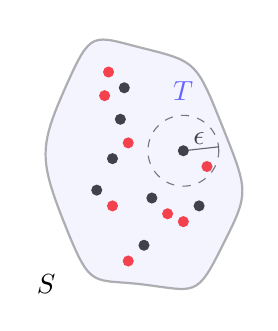
\begin{tikzpicture}
    % Points scattered around
    \foreach \x/\y in {0.5/0.2, -0.3/0.6, 0.1/-0.4, -0.6/-0.3, 0.7/-0.5, -0.4/0.1, -.25/1, 0/-1}
      \fill (\x,\y) circle (2pt);
      % eps-cover scattered around in red
    \foreach \x/\y in {0.8/0.0, -0.5/0.9, 0.3/-0.6, -0.4/-0.5, 0.5/-0.7, -0.2/0.3, -.45/1.2, -.2/-1.2}
    \fill[red] (\x,\y) circle (2pt);

    \draw[dashed, opacity=0.7] (0.5,0.2) circle (0.45);

    % Label the radius epsilon
    \draw[-, opacity=0.8] (0.5,0.2) -- (.95,0.25);
    \node at (0.7,0.35) {$\epsilon$};
    % Smooth curved enclosure around points
    \draw[thick, fill=blue!15, opacity=0.3]
      plot[smooth cycle, tension=1.2] coordinates {
        (1,-1)
        (1.0,0.5)
        (0.0,1.50)
        (-1,1)
        (-1,-0.75)
        (0,-1.5)
      };
  \node at (-1,-1.25)[below left]{$S$};
  \node[blue!60] at (.75,1.2)[below left]{$T$};
  \end{tikzpicture}
  \caption{An \emph{$\epsilon$-cover} (\textcolor{red}{red}) of a subset $T$ of $S$.}
  \label{fig:1}
\end{figure}

\begin{definition}
  The \emph{$\epsilon$-covering number} of $T\subset S$ is
  \begin{equation*}
    N(\epsilon, T, d) = \min\left\{
    \big|\widehat{T}\big| \mid \widehat{T}\text{ is a }\epsilon\text{-cover of T}
    \right\}.
  \end{equation*}
\end{definition}

\begin{definition}
  A set $T$ is \emph{totally bounded} if for all $\epsilon > 0$, $N(\epsilon, T, d) < \infty$. 
\end{definition}
When $d$ is known, we may drop it from the notation $N(\epsilon, T, d)$, or even the set $T$.
\begin{definition}
  The function $\epsilon \mapsto \log{N(\epsilon, T, d)}$ is called the \emph{metric entropy} of $T$.
\end{definition}
\begin{definition}
  If $\lim_{\epsilon \to 0} \frac{\log{N(\epsilon, T)}}{\log(1/\epsilon)}$ exists, it is called the
  \emph{metric dimension} of $T$.
\end{definition}

\begin{example}
  Let $d \in \Z^+$.
  Consider $([0,1]^d, l^\infty)$, the unit $d$-cube endowed the with metric
  induced by the $l^\infty$ norm. We claim that $N(\epsilon, [0,1]^d, l^\infty)
  = \Theta\left(\frac{1}{\epsilon^d}\right)$.
\end{example}

\begin{figure}[ht]
  \centering
    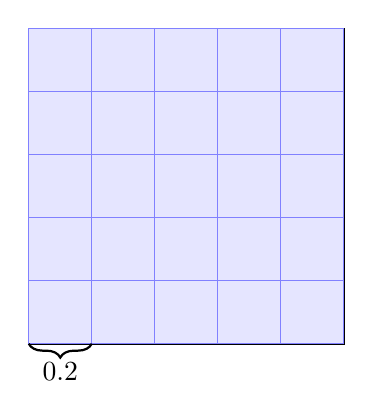
\begin{tikzpicture}
  % Draw the unit square
  \draw[thick] (0,0) rectangle (4,4);

  % Draw the grid with squares of side length 0.2
  \foreach \x in {0,0.8,...,4.0} {
    \foreach \y in {0,0.8,...,4.0} {
      \draw[fill=blue!10, draw=blue!50] (\x,\y) rectangle ++(0.8,0.8);
    }
  }
  
  % Add bracket for side length at bottom left square
  \draw[decorate, decoration={brace, mirror, amplitude=5pt}, thick]
    (0,0) -- (0.8,0) node[midway, yshift=-10pt] {$0.2$};

\end{tikzpicture}
\caption{A $.1$-covering of the unit square $[0,1]^2$ under the $l^\infty$ metric.}
  \label{fig:2}
\end{figure}

See \cref{fig:2}. We can see that when $\epsilon = .1$, a minimal $\epsilon$-cover of $[0,1]^2$ is
given by tiling the square. (It helps that $.2 \mid 1$, in this case.) 
Generalizing to arbitrary $\epsilon > 0$, we can show that
``tiling" the square provides an $\epsilon$-cover with $\lceil \frac{1}{\epsilon}
\rceil^d = \Theta\left(\frac{1}{\epsilon^d}\right)$ 
balls.
So intuitively, \emph{we would expect $d$-dimensional sets in general to have metric dimension $d$,}
or that $N(\epsilon) = \Theta(1/\epsilon^d)$.


\subsection{Packing numbers}
\begin{definition}
  An \emph{$\epsilon$-packing} of a subset $T$ of a pseudometric space $(S,d)$ is a subset 
  $\widehat{T} \subset T$ such that each pair $s,t \in \widehat{T}$ satisfies
  $d(s,t) > \epsilon$. The \emph{$\epsilon$-packing number} of $T$ is 
  $$
  M(\epsilon, T, d) = \max\left\{
    \big|\widehat{T}\big| \mid \widehat{T} \text{ is an }\epsilon\text{-packing of }T 
  \right\}.
  $$
\end{definition}


\begin{figure}[ht]
  \centering
  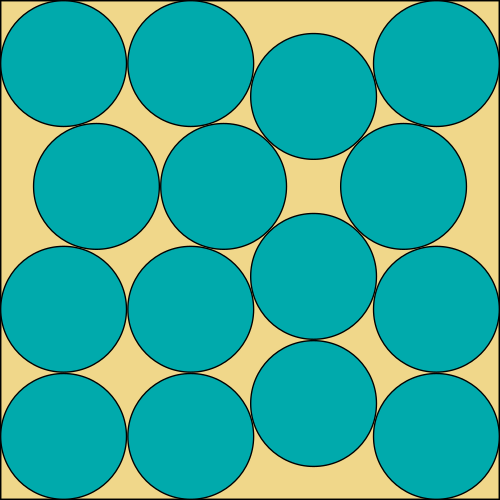
\includegraphics[width=0.2\textwidth]{assets/circle-packing.png}
  \caption{(Not my image.) Let's say this is the unit square, and 
  the metric is induced by the $l^2$ norm. Set our $\epsilon$-packing to be the
  centers of each ball, and say
that each ball has radius $\epsilon$.}
  \label{fig:circle-packing}
\end{figure}
\href{https://en.wikipedia.org/wiki/Circle\_packing}{Circle packing} (in $\R^d$) is a classical problem of packing circles into 
a set (typically connected, with boundary). Famously it was studied by
Lagrange, in his calculus of variations (among other topics). Here we can think
of this definition
as a generalization of this idea.
The notion of covering numbers involves a minimization problem, while the notion of 
packing numbers involves a maximization problem. It turns out that these two quantities are closely
related.
\begin{theorem}
  For all $\epsilon > 0$, $M(2\epsilon) \le N(\epsilon) \le M(\epsilon)$.
\end{theorem}
Thus the scaling of covering and packing numbers is the same.
\begin{proof}
  For the first inequality, consider a minimal $\epsilon$-cover $\widehat{T}$ of $T$. 
  Any two elements of a $2\epsilon$-packing of $T$ cannot be within $\epsilon$ of the same
  element of $\widehat{T}$, otherwise the triangle inequality shows that they are
  within $2\epsilon$ of each other.
  Thus there can be no more than one  element of a $2\epsilon$ packing for each of the
  $N(\epsilon)$ elements of $\widehat{T}$.

  For the second inequality, consider an $\epsilon$-packing $\widehat{T}$ of size $M(\epsilon)$.
  Since it is maximal, no other point $s \in T$ can be added for which some $t\in \widehat{T}$ has
  $d(s,t) > \epsilon$. Thus $\widehat{T}$ is an $\epsilon$-cover, so 
  the minimal $\epsilon$-cover has size $N(\epsilon) \le M(\epsilon)$.
\end{proof}


\begin{example}
  Let $\dabs{\cdot}$ be any norm on $\R^d$, and let $B$ be the unit ball under that norm.
  Then 
  we claim
  $$
  \frac{1}{\epsilon^d} \le N(\epsilon, B, \dabs{\cdot}) \le \left(\frac{2}{\epsilon} + 1\right)^d.
  $$
\end{example}
\begin{proof}
  For the lower bound, let $\{x_1,\ldots, x_N\}$ be an $\epsilon$-cover of size
  $N = N(\epsilon, B)$, 
  and consider that
  $$
  B \subseteq \bigcup_{i=1}^N (x_i + \epsilon B).
  $$
  By countable subadditivity of Lebesgue measure,
  $$
  \mu(B) \le N(\epsilon, B)\mu(\epsilon B) = N(\epsilon, B)\epsilon^d \mu(B),
  $$
  hence
  $N(\epsilon, B) \ge 1/\epsilon^d$.
  For the upper bound, consider a maximal $\epsilon$-packing $\{x_1,\ldots, x_M\}$ of size 
  $M = M(\epsilon, B)$. Since it is a packing, the balls $x_i + (\epsilon / 2)B$ are
  disjoint.
  Each of these balls is contained in $(1+\epsilon / 2)B$. 
  Thus
  $$
\bigcup_{i=1}^M (x_i + \frac{\epsilon}{2}B) \subseteq (1+\epsilon/2)B.
  $$
  Therefore
  by additivity of Lebesgue measure,
  \begin{align*}
    M\mu((\epsilon/2)B) &\le \mu((1+\epsilon/2)B)\\
    \Longrightarrow \left(\frac{\epsilon}{2}\right)^d\mu(B)&\le \left(1+\frac{\epsilon}{2}\right)^d\mu(B).
  \end{align*}
  Hence, $N(\epsilon, B) \le M(\epsilon, B) \le (2/\epsilon + 1)^d$.
\end{proof}
\section{Lipschitz mappings}
  \begin{theorem}
  Let $F$ be a parametrized class of functions
  $$
  F = \{f(\theta, \cdot) \mid \theta \in \Theta\}.
  $$
  Let $\dabs{\cdot}_\Theta$ be a norm on $\Theta$, and let $\dabs{\cdot}_F$ be a norm on $F$.
  Suppose that the mapping $\theta\mapsto f(\theta,\cdot)$ is $L$-Lipschitz, that is
  $$
  \dabs{f(\theta,\cdot) - f(\theta', \cdot)}_F \le L\dabs{\theta - \theta'}_{\Theta}.
  $$
  Then $N(\epsilon, F, \dabs{\cdot}_F)\le N(\epsilon/L, \Theta, \dabs{\cdot}_\Theta).$
  \end{theorem}
  \begin{proof}
    Let's try to prove this live to fill time? Or look it up in the morning.
  \end{proof}

  We care about Lipschitz parametrization as they allow us to translate covers of the parameter space
  into covers of the function space.
  For example, if $F$ is smoothly parametrized by a compact set of $d$ parameters,
  then $N(\epsilon, F) = \mc{O}(1/\epsilon^d)$.
  \begin{example}[1-dimensional Lipschitz functions]
    Let $F$ be the set of $L$-Lipschitz functions mapping from $[0,1] \to [0,1]$. Then
    in the infinity norm $\dabs{f}_\infty = \sup_{x\in [0,1]} \abs{f(x)}$, 
    $$
    \log{N(\epsilon,F,\dabs{\cdot}_\infty)} = \Theta(L/\epsilon).
    $$
  \end{example}
  \begin{proof}[Proof idea]
   Form an $\epsilon$ grid of the $y$-axis, and an $\epsilon/L$ grid of the $x$-axis, and
   consider all functions that are piecewise linear on this grid, where all pieces have slope
   $L$ or $L$. There are $1/\epsilon$ starting points, and for each starting point,
   there are $2^{L/\epsilon}$ slope choices. It remains to show that this set is an $\mc{O}(\epsilon)$
   packing and an $\mc{O}(\epsilon)$ cover.
  \end{proof}
  \begin{example}
    Let $F_d$ be the set of $L$-Lipschitz functions wrt $\dabs{\cdot}_\infty$, this time mapping from $[0,1]^d$
    to $[0,1]$. Then
    $$
    \log{N}(\epsilon, F_d,\dabs{\cdot}_\infty) = \Theta((L/\epsilon)^d).
    $$
    Note the exponential dependence on the dimension.
  \end{example}
  \section{Johnson-Lindenstrauss lemma and its optimality}
  Many famous people have worked on Johnson-Lindenstrauss, including Noga Alon, and Terrence Tao.
  Alon brought a combinatorial approach towards JL, while it seems Tao focuses on JL's applications to 
  signal reconstruction in ``\emph{compressed sensing}."
  \begin{theorem}[Johnson-Lindenstrauss lemma]
    Let $X \subset \R^d$ be any set of size $n$, and let $\epsilon \in (0,1/2)$ be arbitrary.
    Then there exists a map $f : X \to \R^m$ for some $m = \mc{O}(\epsilon^{-2}\log{n})$ such that
    \begin{equation*}
      \forall x,y\in X, \quad (1-\epsilon)\dabs{x-y}_2^2 \le \dabs{f(x)-f(y)}_2^2 \le (1+\epsilon)\dabs{x-y}_2^2.\tag{1}
    \end{equation*}
  \end{theorem}
  JL lemma is a so-called bi-Lipschitz embedding, in a finite setting. An elegant and short proof of
  this theorem uses the probabilistic
  method of combinatorics, made famous by Alon and Erd\"os.
  In the original JL paper, it was proven for any $\epsilon < 1/2$, there exists $n$ point sets
  $X\subset \R^n$ for which any embedding $f : X \to \R^m$ satisfying (1) must have
  $m = \Omega(\log{n})$. Alon and Levenshtein later showed the existence of an $n$ point
  set $X \subset \R^n$ such that any $f$ satisfying (1) must have 
  $m = \Omega(\min\{n, \epsilon^{-2}\log{n}/\log{(1/\epsilon)}\}).$
  Larson and Nelson\footnote{Nelson is chair at UC Berkeley CS now.} prove the following result settling the optimality
  of the JL lemma, for almost the full range of $\epsilon$.
  \begin{theorem}
    For any integers $n,d \ge 2$, and $\epsilon \in (\log^{0.5001}{n/ \sqrt{\min\{n,d\}}}, 1)$, there exists
    a set of points $X \subset \R^d$ of size $n$ such that any map $f : X \to \R^m$ providing (1)
    must have $$
    m = \Omega(\epsilon^{-2}\log(\epsilon^2n)).
    $$
  \end{theorem}
  Their proof uses covering numbers, but it is too long to cover in this presentation.
  This should conclude this presentation.
  \nocite{*}
  \bibliographystyle{unsrt}
  \bibliography{refs}
\end{document}




